\documentclass[12pt,a4paper,oneside,titlepage] {article}

\usepackage[T2A]{fontenc}
\usepackage[utf8]{inputenc}
\usepackage[russian]{babel}
\usepackage{hyperref}
\usepackage{multicol}
\usepackage{listings}
\usepackage{geometry}
\usepackage{minted}

\usepackage{graphicx}
\graphicspath{ {./images/} }
\usepackage{wrapfig}

\begin{document}

% НАЧАЛО ТИТУЛЬНОГО ЛИСТА
\begin{center}
  \hfill 
  \break
  \textbf{
    \footnotesize{Министерство науки и высшего образования Российской Федерации}\\
    \hfill \break
    \footnotesize{Федеральное государственное бюджетное образовательное учреждение высшего образования}\\
    \small{«МОСКОВСКИЙ ГОСУДАРСТВЕННЫЙ ТЕХНИЧЕСКИЙ УНИВЕРСИТЕТ имени Н.Э.БАУМАНА\\(национальный исследовательский университет)»}}\\
    \footnotesize{(МГТУ им. Н.Э. Баумана)}\\
    \includegraphics[width=25mm,scale=0.25]{emblem}
\end{center}
\hfill 
\break
\normalsize{Факультет: Информатика и системы управления}\\
\hfill \break
\normalsize{Кафедра: Теоретическая информатика и компьютерные технологии}\\
\hfill\break
\begin{center}
  \textbf{\large{Лабораторная работа №1}}\\
  \large{Настройка среды разработки Java}\\
  \textbf{\large{Вариант №0}}\\
\end{center}
\hfill \break
\hfill \break
\hfill \break
\hfill \break
\hfill \break
\hfill \break
\hfill \break
\hfill \break
\begin{flushright}
  \normalsize{
    Выполнил\\
    студент группы ИУ9-21Б\\
    Лисов Алексей
  }
\end{flushright}

\hfill \break
\begin{center} Москва, 2023 \end{center}
\thispagestyle{empty} % выключаем отображение номера для этой страницы
% КОНЕЦ ТИТУЛЬНОГО ЛИСТА

\section{Условие}
Для освоения языка программирования Java требуется реализовать интерфейс для обеспечения возможности полиморфной обработки объектов класса. Реализовать интерфейс Comparable<T> и переопределить метод toString. Условие задачи, исходный код и пример работы программы необходимо прислать в формате \LaTeX.

\section{Код решения}
Файл Main.java
\begin{minted}{java}
import java.util.Arrays;

public class Main {
    public static void main(String[] args) {

        Fraction[] a = new Fraction[] {
                new Fraction(6, 5),
                new Fraction(2, 2),
                new Fraction(2, 2),
                new Fraction(1, 2),

        };
        System.out.println(a[1].compareTo(a[2]));

        Arrays.sort(a);

        for (Fraction s : a) {
            System.out.println(s);
        }
    }
}
\end{minted}
Файл Fraction.java
\begin{minted}{java}
public class Fraction implements Comparable<Fraction> {
    public int ch, zn;

    public Fraction(int ch_, int zn_) {
        this.ch = ch_;
        this.zn = zn_;
    }

    @Override
    public String toString() {
        return "Fraction {"
                + "Числитель='" + this.ch + '\''
                + ", Знаметель='" + this.zn
                + "'}";
    }

    @Override
    public int compareTo(Fraction o) {
        return (this.ch * o.zn) - (o.ch * this.zn);
    }
}
\end{minted}

\section{Пример работы программы}
\begin{figure}[H]
    \centering
    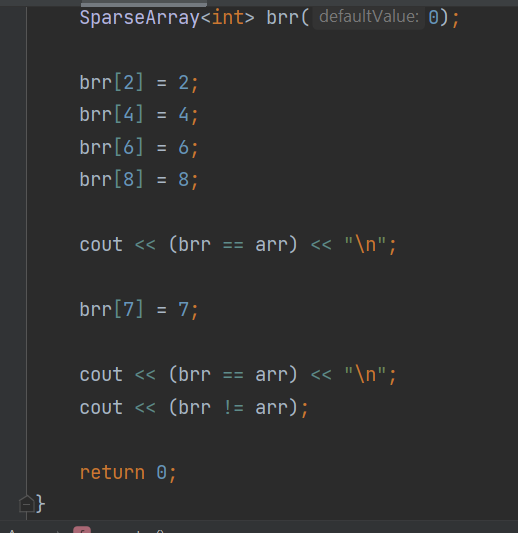
\includegraphics[width=\linewidth]{image.png}
    \caption{Вывод программы}
    \label{fig:my_label}
\end{figure}


\end{document}
